\chapter{Systemarkitektur}\label{kapitel_Systemark}

\begin{longtabu} to \linewidth{@{}l l l X[j]@{}}
    Version &    Dato &    Ansvarlig &    Beskrivelse\\[-1ex]
    \midrule
    0.1 &    4/11-15 &    Alle &    Tilføjelse af arkitektur\\
    Tekst &    Tekst &    Tekst &    Tekst\\
    Tekst &    Tekst &    Tekst &    Tekst.\\
    Tekst &    Tekst &    Tekst &    Tekst.\\
\label{version_Systemark}
\end{longtabu}

\textbf{Formål}\\
Til beskrivelse af systemarkitekturen og det detaljerede design for produktet, er der benyttet SysML.
SysML anvendes her, da blodtryksmålesystemet både indeholder software og hardware. Et af de  
vigtigste argumenter for brug af SysML er, at de fastlagte standarder i sproget medfører en bedre 
formidling af systemet, hvilket giver et større overblik.


\section{Hardware}
Hardware-delen består af et elektronisk kredsløb, som forstærker signalet fra tryktransduceren og filtrerer det med et indbygget analogt filter.\\
\newline
Til at skabe overblik over blodtryksmålesystemets hardware er der uarbejdet en figur, der viser hele det overordnet system.

\begin{figure}[H]
\centering
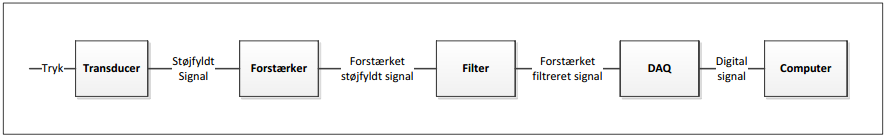
\includegraphics[scale=0.65]{so.PNG}
\caption{Blodtryksmålersystemet}
\end{figure}

Denne illustrerer, at der ind i transduceren kommer tryk og ud kommer et støjfyldt signal. Dette signal bliver ved forstærkeren forstærket og heraf et forstærket støjfyldt signal. Igennem filtret bliver støjen filtreret fra. Det filtrerede signal føres igennem DAQ’en, som omdanner det til et digitalt signal, som anvendes i computerens softwareprogram.\\
\newline
Til at præcisere komponenterne i blodtryksmålesystemets hardware, er der valgt at lave strukturdiagrammer. Her er der anvendt blokdefinitionsdiagram (BDD) og et internt blokdiagram (IBD).

\subsection{BDD}
BDD'et er anvendt til, at dokumentere nedbrydningen af systemet og forholdene mellem blokkene.  

\begin{figure}[H]
\centering
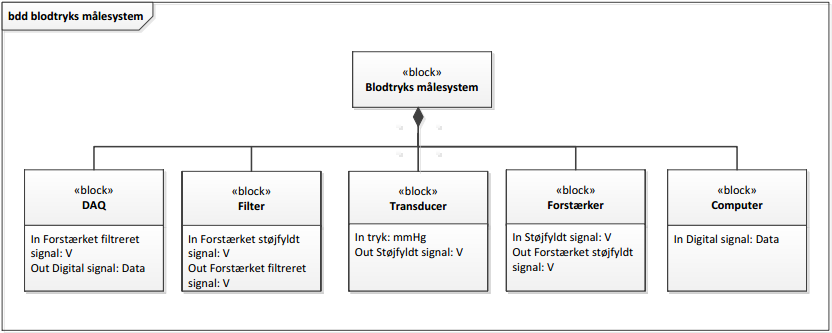
\includegraphics[scale=0.80]{bdd.PNG}
\caption{BDD}
\end{figure}

\textbf{Blokbeskrivelser:}
\begin{itemize}
\item Transducer: En tryktransducer, som konverterer et tryk til et analogt elektrisk signal
\item Forstærker: Signalet forstærkes således at hele forsyningsspændingen udnyttes
\item Filter: Et 2. ordens lavpasfilter fjerner højfrekvent støj
\item DAQ: A/D konverter omsætter den analoge indgangsspænding til et digitalt signal
\item Computer: Enheden som indeholder softwareprogrammet til visning af blodtryk
\end{itemize}

\newpage

\subsection{IBD}
IBD'et er anvendt til, at dokumentere den interne struktur i blokkene.
\begin{figure}[H]
\centering
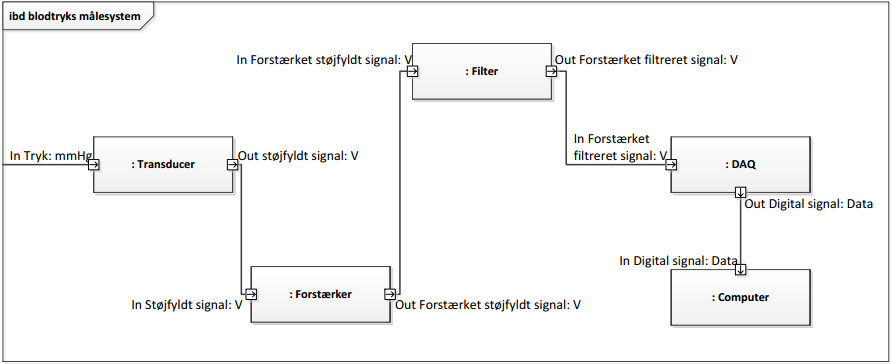
\includegraphics[scale=0.75]{ibd.PNG}
\caption{IBD}
\end{figure}

\subsubsection{Signalbeskrivelse}

\begin{longtabu} to \linewidth{@{}l l X[j]@{}}
    \textbf{Forbindelse} &    \textbf{Signaltype} &    \textbf{Funktionalitet}\\[-1ex]
    \midrule
    Transducer - forstærker &    Støjfyldt signal &    Elektrisk analogt signal med støj i enheden volt\\
    Forstærker - filter &    Forstærket støjfyldt signal &    Elektrisk analogt forstærket støjfyldt signal i enheden volt\\
    Filter - DAQ &    Forstærket filtreret signal &    Elektrisk analogt forstærket filtreret signal i enheden volt\\
    DAQ - computer &   Digitalsignal &    Elektrisk digitalt signal med data via USB\\
    Batterier - transducer, forstærker, filter	&		Forsyningsspænding	&	Positiv og negativ 9V\\
\label{version_Signaltabel}
\end{longtabu}

\newpage

\section{Software}
Brugergrænsefladen i software-delen består af to forskellige GUI'er, en til at logge ind og en til diagnostik. Programmet indeholder en række klasser indeholdende funktionaliteten beskrevet i UC's samt databaser til opbevaring af data. Softwaren er opbygget af trelagsmodellen. \\
\newline
For at skabe et overblik over sammenhængen mellem UC's og softwaren i systemet, er der udviklet en applikationsmodel. Applikationsmodellen indeholder en domænemodel over hele systemet, et klassediagram for hver enkelt UC, et sekvensdiagram over hele systemet, et sekvensdiagram for hver UC og et opdateret klassediagram med metoder. Ved at opdele de forskellige dele i softwaren samt at oprette klasser efter den ønskede funktionalitet i UC's, opnås en sammenhænge og overskuelighed over systemet som helhed.


\subsection{Domænemodel}
Domænemodellen er udviklet vha. navneordsanalyse i de fem UC's. Domænemodellen giver et overblik over hvilken funktionalitet der - ud fra UC's - er relevant. Funktionaliteterne er opdelt i kasser, der senere bliver til klasser i softwaren. 

\begin{figure}[H]
\centering
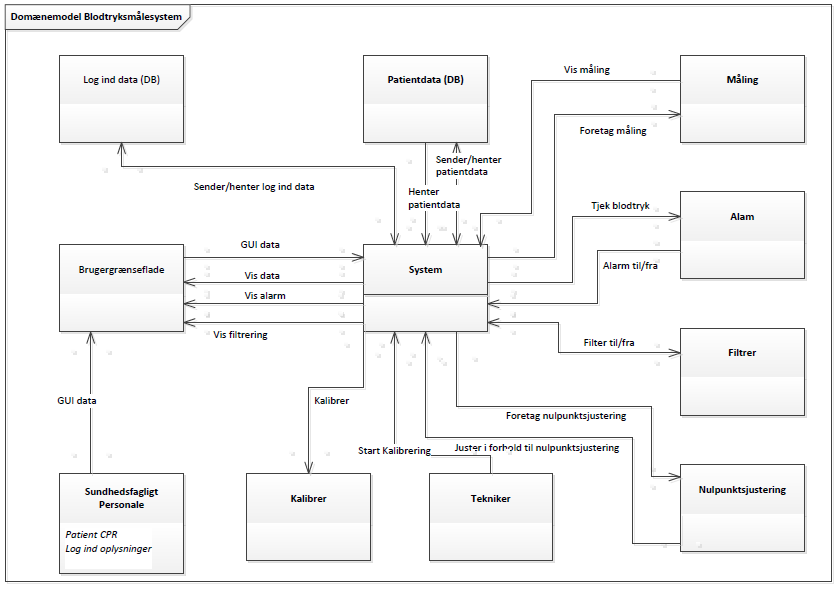
\includegraphics[scale=0.70]{dom.PNG}
\caption{Domænemodel blodtryksmålersystem}
\end{figure}

\newpage

\subsection{Klassediagram}
Klassediagrammerne for hver enkelt UC viser sammenhængen mellem de forskellige instanser i den enkelte UC. \newline 
\textit{Boundary-klasser} er den akutuelle UC's aktører. \newline 
\textit{Controller-klassen} indeholder UC'ens funktionalitet og udfører UC'en ved at interagere med boundary-klasserne og domain-klasserne. Controller-klassen er opkaldt efter den aktuelle UC's navn. \newline
\textit{Domain-klassen} repræsenterer systemets domæne og hukommelse. 
%------------UC1----------------------------
\subsubsection{Klassediagram UC1}
I klassediagrammet for UC1 logger sundhedsfagligt personale ind vha. brugergrænsefladen - de er begge to boundary-klasser. Brugergrænsefladen sender besked til controller-klassen "Log ind". Log ind-data hentes - via controlleren - i Log ind databasen og sendes tilbage til brugergrænsefladen via controlleren, hvorved sundhedsfagligt personale logges ind. 
%Metoder og attributter er opdateret efter konstruering af sekvensdiagram.
\begin{figure}[H]
\centering
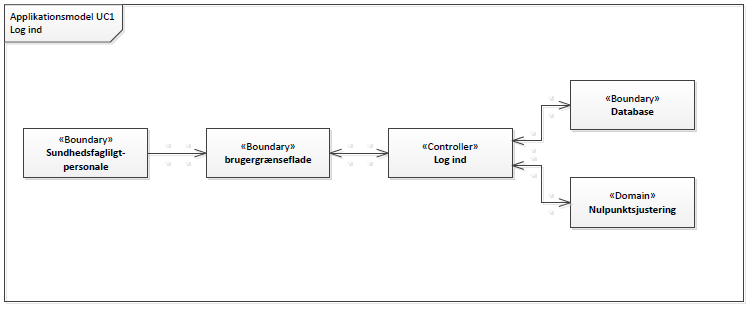
\includegraphics[scale=0.70]{app1.PNG}
\caption{Applikationsmodel UC1}
\end{figure}

%------------------UC2------------------------
\subsubsection{Klassediagram UC2}
I klassediagrammet for UC2 er sundhedsfagligt personale og brugergrænsefladen boundary-klasser. "Hent patientoplysninger" er UC'ens controller-klasse. Patientoplysningerne hentes fra Patient databasen - en boundary-klasse - og sendes tilbage igennem controller-klassen til brugergrænsefladen. 
\begin{figure}[H]
\centering
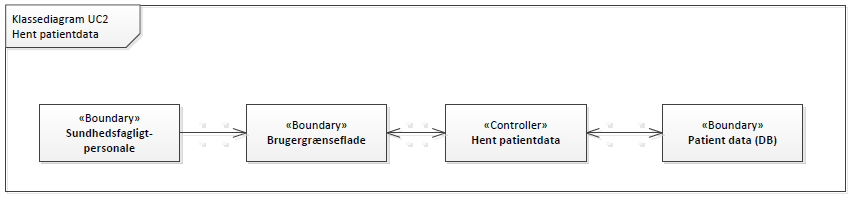
\includegraphics[scale=0.70]{app2.PNG}
\caption{Applikationsmodel UC2}
\end{figure}

\newpage

%------------------UC3------------------------
\subsubsection{Klassediagram UC3}
I klassediagrammet for UC3 er sundhedsfagligt personale og brugergrænsefladen boundary-klasser. "Nulpunktsjuster"\ er UC'ens controller-klasse, som udfører UC'en vha. domain-klassen "Nulpunktsjustering". Nulpunktsjusteringen sendes tilbage til brugergrænsefladen fra domain-klassen, igennem controller-klassen.
\begin{figure}[H]
\centering
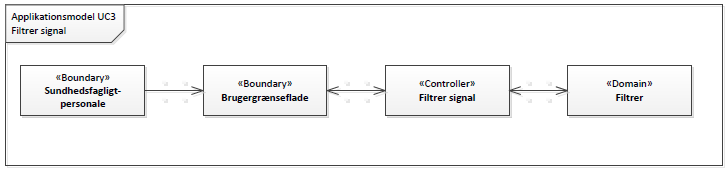
\includegraphics[scale=0.70]{app3.PNG}
\caption{Applikationsmodel UC3}
\end{figure}

%------------------UC4------------------------
\subsubsection{Klassediagram UC4}
I klassediagrammet for UC4 er brugergræsnefladen boundary-klasse. "Alarmer"\ er UC'ens controller-klasse, som sender besked omkring alarmering til domain-klassen "Alarm"\. Domain-klassen alarmerer, og sender alarmen til brugergrænsefladen via controller-klassen.
\begin{figure}[H]
\centering
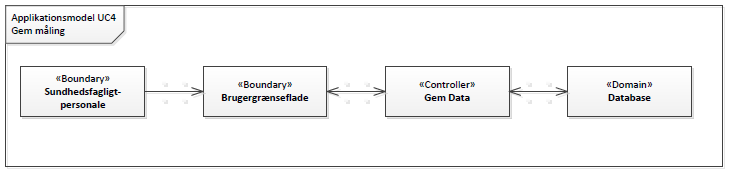
\includegraphics[scale=0.70]{app4.PNG}
\caption{Applikationsmodel UC4}
\end{figure}

%------------------UC5------------------------
\subsubsection{Klassediagram UC5}
Klassediagrammet for UC4 viser, at sundhedsfagligt personale og brugergrænsefladen er boundary-klasser. "Filtrer signal"\ er UC'ens controller-klasse som får besked fra brugergrænsefladen om at filtrere signalet - og sender filtreringen tilbage til brugergrænsefladen.  
\begin{figure}[H]
\centering
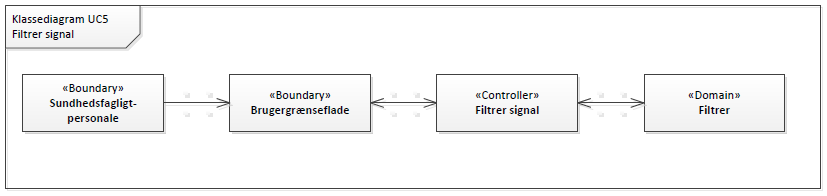
\includegraphics[scale=0.70]{app5.PNG}
\caption{Applikationsmodel UC5}
\end{figure}

%------------------UC6------------------------
\subsubsection{Klassediagram UC6}
I klassediagrammet for UC5 er sundhedsfagligt personale og brugergrænsefladen boundary-klasser. "Gem måling"\ er UC'ens controller-klasse, som får besked fra brugergrænsefladen om at gemme den akutelle måling. Denne information sendes videre til domain-klassen "Patientdata"\, som sender besked tilbage til brugergrænsefladen, igennem controller-klassen om, at data er gemt.
\begin{figure}[H]
\centering
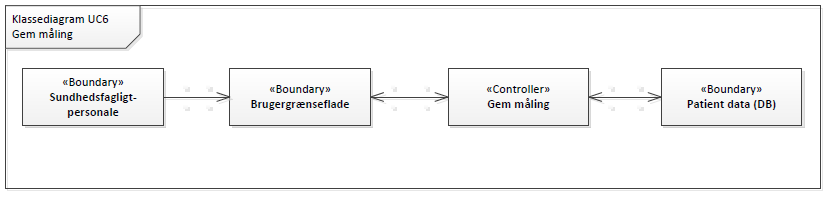
\includegraphics[scale=0.70]{app6.PNG}
\caption{Applikationsmodel UC6}
\end{figure}


%------------------UC7------------------------
\subsubsection{Klassediagram UC7}
I klassediagrammet for UC6 ses det, at tekniker og brugergrænsefladen er boundary-klasser. Teknikeren kalibrerer systemet i controller-klassen, som justerer brugergrænsefladen i forhold til kalibreringen. 
\begin{figure}[H]
\centering
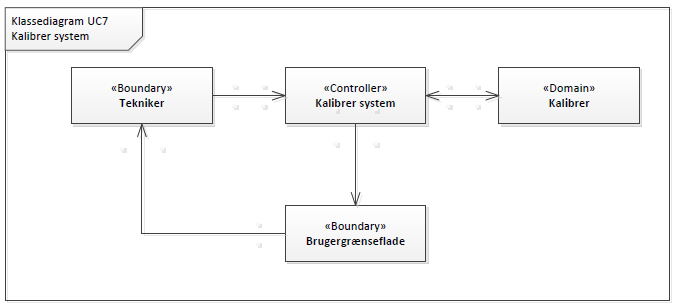
\includegraphics[scale=0.70]{app7.PNG}
\caption{Applikationsmodel UC7}
\end{figure}

\newpage

\subsection{Sekvensdiagram}

Controlleren i sekvensdiagrammerne er logiklaget, hvor domainklasserne er klasser tilkoblet logiklaget.

%------------------UC1------------------------
\subsubsection{Sekvensdiagram UC1}
Sekvensdiagrammet for UC1 viser, at sundhedsfagligt personale indtaster Log ind data i brugergrænsefladen. Disse behandles - vha. metoden TjekLogInd() - i controlleren Log Ind. Dataen hentes i databasen - vha. getLogIndData() - Log Ind data og sendes tilbage til controlleren og tjekkes heri. Er oplysningerne korrekte, vises Diagnostik-GUI'en. \\
Der er en alternativ rute, hvor de indtastede oplysninger er forkerte. Dette vises i LogInd-GUI'en, og bruger indtaster oplysningerne forfra.
\begin{figure}[H]
\centering
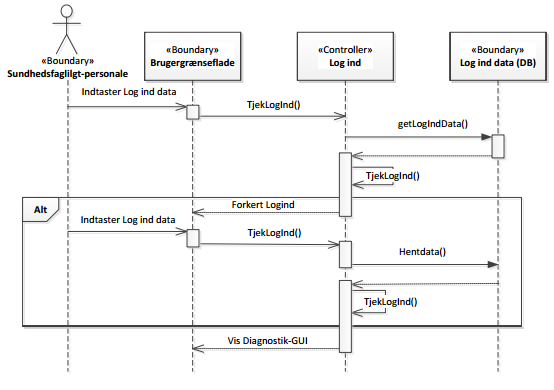
\includegraphics[scale=0.70]{sd1}
\caption{Sekvensdiagram UC1}
\end{figure}

%------------------UC2------------------------
\subsubsection{Sekvensdiagram UC2}
I diagrammet for UC2 ses det, at sundhedsfagligt personale indtaster patientens CPR i brugergrænsefladen. Patienten tjekkes i controlleren vha. TjekCPR(). Data hentes fra Patient data - vha. getPatientdata() - og sendes tilbage til controlleren, som tjekker disse. \\
Den alternative rute består i, at det indtastede CPR er forkert. I det tilfælde, sendes en besked til brugeren herom, og der kan ske en ny indtastning.
\begin{figure}[H]
\centering
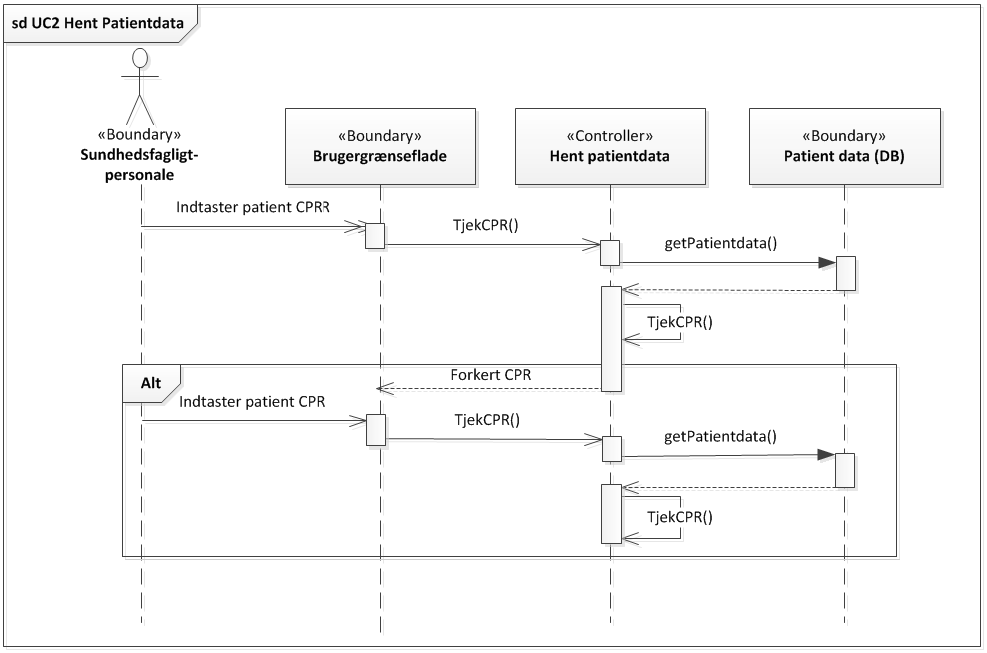
\includegraphics[scale=0.70]{sd2}
\caption{Sekvensdiagram UC2}
\end{figure}

%------------------UC3------------------------
\subsubsection{Sekvensdiagram UC3}
Diagrammet for UC3 viser at sundhedsfagligt personale, igennem brugergrænsefladen, beder om at få systemet nulpunktsjusteret. Nulpunktjusteringen sendes som besked fra brugergrænsefladen til controlleren via metoden NulpunktsJuster(). Denne metode sendes videre til Nulpunktsjustering-klassen, som sender en besked, igennem controlleren, til brugergrænsefladen om, at blodtryksmålingen skal vises i brugergrænsefladen.
\begin{figure}[H]
\centering
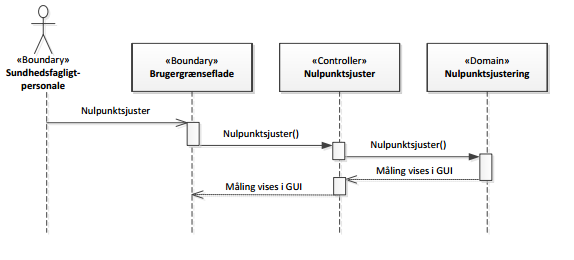
\includegraphics[scale=0.70]{sd3.PNG}
\caption{Sekvensdiagram UC3}
\end{figure}

%------------------UC4------------------------
\subsubsection{Sekvensdiagram UC4}
I diagrammet beder controlleren ved hjælp af metoden Alarm() om at Alarm-klassen skal tjekke op på om alarmfunktionen skal slås til eller fra. Efter metoden Alarm() er kørt gives der besked tilbage til controlleren og videre til brugergrænseflade, hvor man ville kunne se om amarmen er slået til eller fra.
Efterfølgende kan der forekomme en alternativ funktion, hvor brugeren ved hjælp af lydløsknappen på brugergrænsefladen kan slå lydløs funktionen til. Når brugeren har trykket på knappen, starter controlleren metoden Lydløs(), som sender videre besked om at blive kørt i Alarm-klassen. Der sendes en returbesked tilbage til gennem controlleren og videre til brugergrænsefladen.

I sekvensdiagrammet over UC4 ses det, at det er controlleren der sætter alarmen igang så snart blodtryksværdierne er udenfor de angivne grænseværdier. 
\begin{figure}[H]
\centering
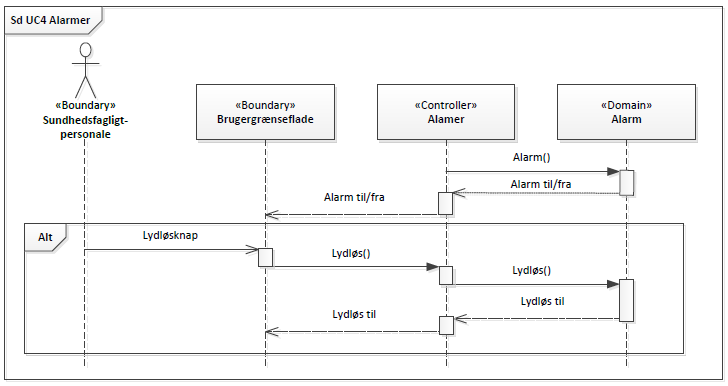
\includegraphics[scale=0.70]{sd4.PNG}
\caption{Sekvensdiagram UC4}
\end{figure}

%------------------UC5------------------------
\subsubsection{Sekvensdiagram UC5}
Sundhedsfagligt personale trykker på til/fra-knappen i brugergrænsefladen. Metoden Filtrer() i controllerklassen giver besked om at Filtrer() skal kørers i Domainklassen ”Filter”. Der gives efterfølgende besked til controllerklassen og videre til brugergrænsefladen, hvor der kan ses ved hjælp af en radiobutton om filteret er slået til eller fra.
\begin{figure}[H]
\centering
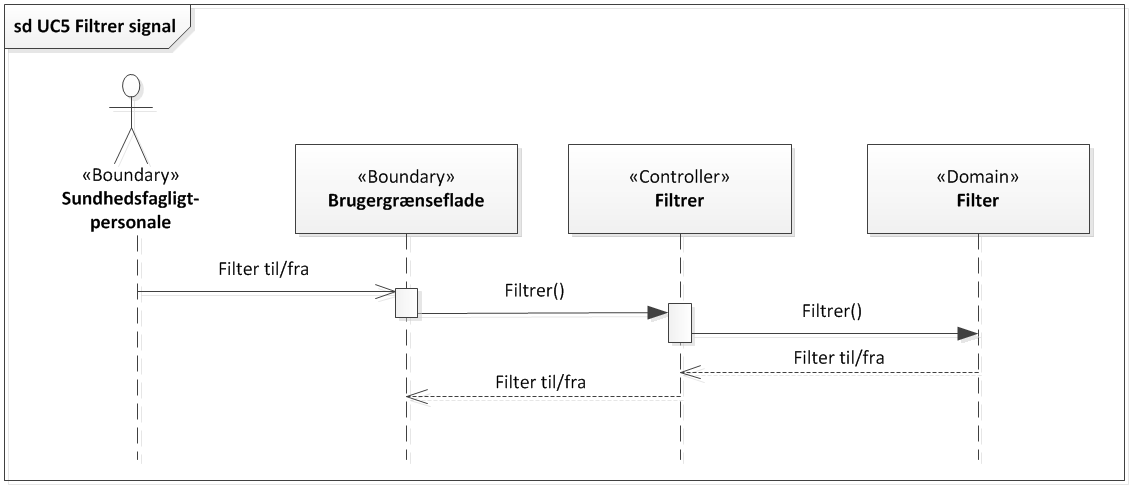
\includegraphics[scale=0.70]{sd5.PNG}
\caption{Sekvensdiagram UC5}
\end{figure}

%------------------UC6------------------------
\subsubsection{Sekvensdiagram UC6}
Sundhedsfagligt personale trykker på gem knap i brugergrænsefladen. Dette aktiverer metoden GemBlodtryksdata() i controlleren, som giver videre besked til at køre den i boundaryklassen ”Patient Data (DB)”. Hvis der sker en fejl under gemmeprocessen og målingen dermed ikke bliver gemt, vil et alternativt handlingsforløb indtræde. ”Patient data (DB) ” vil i dette tilfælde give en returbesked til controlleren og videre til brugergrænsefladen, som meddeler til det sundhedsfaglige personale at målingen ikke er gemt. Herefter vil det sundhedsfaglige personale kunne prøve igen. 
Er målingen gemt, vil der blive givet besked til controlleren fra ”Patient data (DB)”, som videre vil give besked til brugergrænsefalden. 

\begin{figure}[H]
\centering
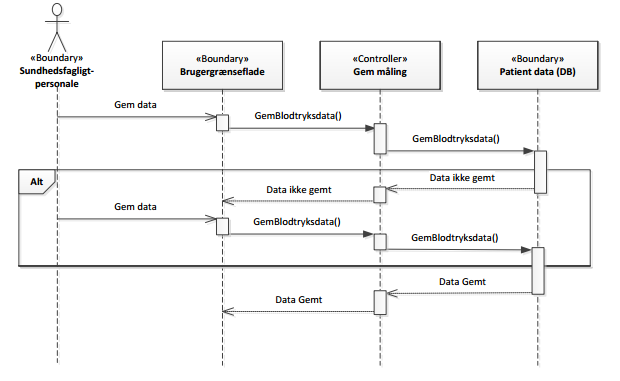
\includegraphics[scale=0.70]{sd6.PNG}
\caption{Sekvensdiagram UC6}
\end{figure}

%------------------UC7------------------------
\subsubsection{Sekvensdiagram UC7}
I diagrammet ses det at teknikeren starter med at påtrykke et kendt tryk i controlleren. Dette vil starte metoden Kalibrer() i Domainklassen ”Kalibrer”. ”Kalibrer” giver besked om afvigelser til controlleren. I tilfælde at der ikke er nogen afvigelser gives der besked om dette og teknikeren fortager ikke nogen ændringer. Ved afvigelser justere teknikeren det ved hjælp af ”Kalibrer”-klassen og der gives direkte besked tilbage til brugergrænsefladen om ændringerne.            
\begin{figure}[H]
\centering
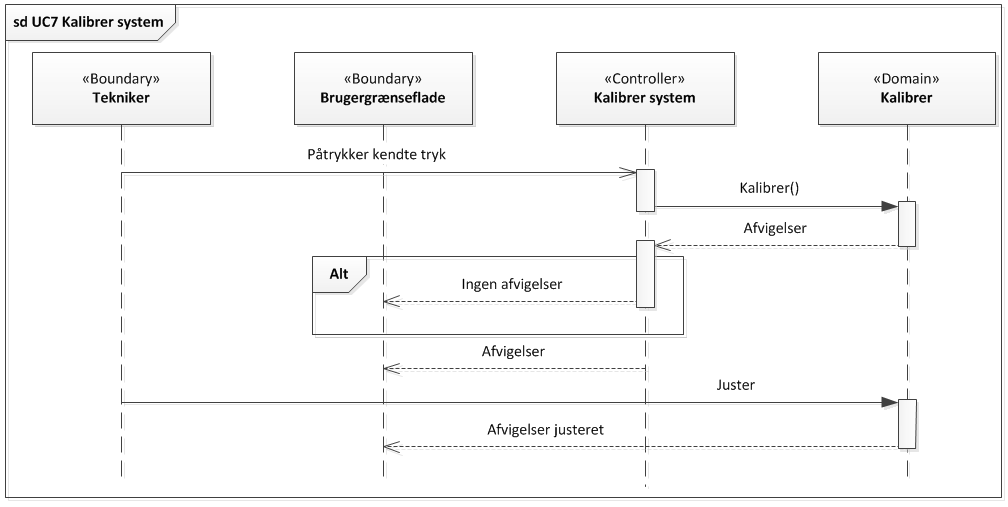
\includegraphics[scale=0.70]{sd7.PNG}
\caption{Sekvensdiagram UC7}
\end{figure}

\chapter{Design}\label{kapitel_Design}

\begin{longtabu} to \linewidth{@{}l l l X[j]@{}}
    Version &    Dato &    Ansvarlig &    Beskrivelse\\[-1ex]
    \midrule
    0.1 &    6/11-15 &    SV &    Tilføjelse af arkitektur\\
    0.2 &    11/11-15 &    SV &    Tilføjelse af design\\
    Tekst &    Tekst &    Tekst &    Tekst.\\
    Tekst &    Tekst &    Tekst &    Tekst.\\
\label{version_Design}
\end{longtabu}

\textbf{Formål}
I dette kapitel er design af SW og HW illustreret med figurer og forklaret.

\section{Designproces (GUI)}
I udvikling af projektets brugergrænseflader er der brugt generelle principper om gode brugergrænseflader, MMI. Det er specielt prioriteret at brugeren skal være i kontrol, og at brugerens sprog skal være det gennemgående, da sproget gerne skal ligge til brugerens logik og ikke udviklerens. Brugergrænsefladen er udviklet med sigende knapper, radiobuttons, labels og tekstbokse. \\
\newline
Efter et besøg på dagkirurgisk afsnit på Aarhus Universitets Hospital, Skejby, er brugergrænsefladen forsøgt udviklet således at den passer til brug på en operationsstue. Ideelt set skulle der være to forskellige skærme, og dermed to forskellige brugergrænseflader - én til indtastning af brugeroplysninger og patientdata, og én til diastolisk,- systolisk- og pulsmåling. Brugergrænsefladen med patientoplysninger er til anæstesisygeplejerske/læge hvor brugergrænsefladen indeholdende målinger er til kirurgen. Kirurgens brugergrænseflade skal være simpel og indeholde så få oplysninger som muligt. Denne skal også have en alarmeringsfunktion, som kan sættes på lydløs i eksempelvis tre minutter. Anæstesisygeplejerskens brugergrænseflade skal indeholde mange (nødvendige) informationer om patienten, og skal derfor opbygges så dette er overskueligt.\\
Ud fra den erfarede viden på Dagkirurgisk Afsnit, er det besluttet at sammensmelte de to omtalte skærme, men dog udvikle to forskellige brugergrænseflader. Den første brugergrænseflade indeholder bruger log ind, og en fejlmelding hvis de indtastede data er forkerte. Den anden brugergrænseflade indeholder patientdata samt målingen med de nødvendige informationer og funktioner. For at brugergrænsefladerne skal kunne udgøres for de to skærme på operationstuen, er disse gjort overskuelige og selvsigende. \\
\newline
\textit{Feedback to user}\\
Feedback til brugeren skal gives for, at bruger kan se om en evnetuel kommando er forstået. Hvis ikke der er noget feedback efter en given kommando, ved brugeren ikke, om kommandoen er forstået eller accepteret - og tror dermed, at der er fejl i systemet. En sådan feedback skal have kort reponstid og/eller et \textit{arbejder}-symbol som viser at systemet bearbejder kommandoen.\\
Feedback til brugeren er implementeret således, at der eksempelvis kommer en pop-up meddelelse ved forkert log ind. Når bruger logger ind, skifter brugergrænsefladen hurtigt, så brugeren ved, at handlingen er accepteret.  ....  

\textit{Never interrupt the user}\\
Brugeren skal aldrig forstyrres unødvendigt. Eksempelvis pop-up vinduer, som bruger ikke selv har bedt om, er forstyrrende. De forstyrrende elementer flytter brugers fokus, sætter bruger ud af kontrol og bryder brugers koncentration. Dog kan advarsler være vigtige, og dem af helt vigtig karakter, kan være nødvendig som pop-up. Advarsler af mindre vigtig karakter, kan opstå som pop-up ikoner i et hjørne - uden brug af lyde, pop-up eller andet - så bruger kan reagere når hen ikke længere er fuldt optaget.\\
HVORDAN ER DET IMPLEMENTERET?

\textit{The user should be in control}\\
Brugeren skal lave kommandoerne og systemer skal adlyde disse, og ikke omvendt. Dette kan eksempelvis være en dialogbox på computer med knapperne "OK"\ til at acceptere, "Cancel"\ hvis bruger fortryder og "Help"\ hvis bruger har brug for hjælp.\\
HVORDAN ER DET IMPLEMENTERET?

\textit{Speak the users language}\\


\textit{Design should reflect the user's logic, not the constructor's logic}\\
\newline
\textit{The design of a button should reflect its importance}\\
\newline

  
    

\section{Hardware}
\subsubsection{Lavpasfilter}
Der benyttes et lavpasfilter for at undgå aliasering. Dette kaldes derfor for et antialiseringsfilter.
I dette projekt arbejdes med et aktivt 2. ordens lavpasfilter, som består af et pasbånd og et stopbånd. 

\begin{figure}[H]
\centering
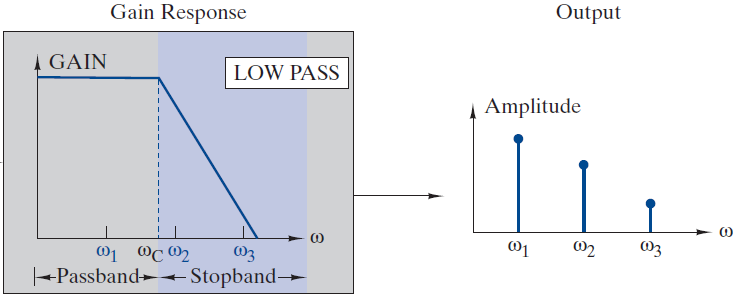
\includegraphics[scale=0.50]{lavpas.PNG}
\caption{Gain respons lavpas}
\end{figure}

Pasbåndet lader lave frekvenser passere igennem med ingen eller uvæsentlig dæmpning, og stopbåndet dæmper høje frekvenser væsentligt. Kurvens udvikling ses på bodeplot med frekvensen i rad/s ud af x-aksen og forstærkning i dB op ad y-aksen. \\
\newline
Knækfrekvensen er overgangen mellem pas- og stopbånd. Med andre ord så er knækfrekvensen, hvor indgangssignalet er dæmpet med 3 dB. \\
\newline
I projektet designes filtret med en knækfrekvens på 50 Hz. Operationsforstærkeren er af typen OP27. Kondensatoren C2 er givet til 680 nF og endvidere R1 = R2. 

\begin{figure}[H]
\centering
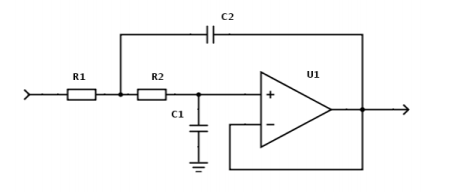
\includegraphics[scale=0.60]{opamp.PNG}
\caption{Unity 2. ordens sallen-key lavpas konfiguration}
\end{figure}

Til at bestemme komponentværdier er der taget udgangspunkt i knækfrekvensen:
$$f_c=\frac{1}{2 \pi \sqrt{C1 \cdot C2 \cdot R1 \cdot R2}} = \frac{1}{2 \pi \sqrt{C1 \cdot C2 \cdot R^2}}$$
Herudfra bestemmes R1 og R2:
$$solve(50=\frac{1}{2 \pi \sqrt{10^{-6} \cdot (680 \cdot 10^{-9}) \cdot R^2}},R)$$
$$R=3860 \ \Omega \approx 3,9 \ k \Omega$$
C1 bestemmes til $1 \ \mu F$
Overføringsfunktionen:
$$T_v(s)=\frac{\frac{1}{R1 \cdot C1 \cdot R2 \cdot C2}}{s^2+s(\frac{1}{R2 \cdot C1}+\frac{1}{R1 \cdot C1})+\frac{1}{R1 \cdot C1 \cdot R2 \cdot C2}}$$

$$T_v(s)=\frac{\frac{1}{(3900(1 \cdot 10^{-6}) \cdot 3900  (680 \cdot 10^{-9}))}}{(s^2+(s(\frac{1}{3900(1 \cdot 10^{-6})}+ \frac{1}{3900(1 \cdot 10^{-6})}))+\frac{1}{(3900(1 \cdot 10^{-6}) \cdot 3900 (680 \cdot 10^{-9})}))}$$

$$T_v(s)=\frac{1}{\frac{25857}{2500000000}s^2 + \frac{663}{125000}s+1}$$

$$T_v(s)=\frac{96685,6170476}{s^2+512,820512821 \cdot s+96685,6170476}$$

Optegner bodeplot vha. værktøj i Maple:
$$sys := TransferFunction(\frac{96685,6170476}{s^2+512,82 \cdot s + 96685,6170476}):$$

\begin{figure}[H]
\centering
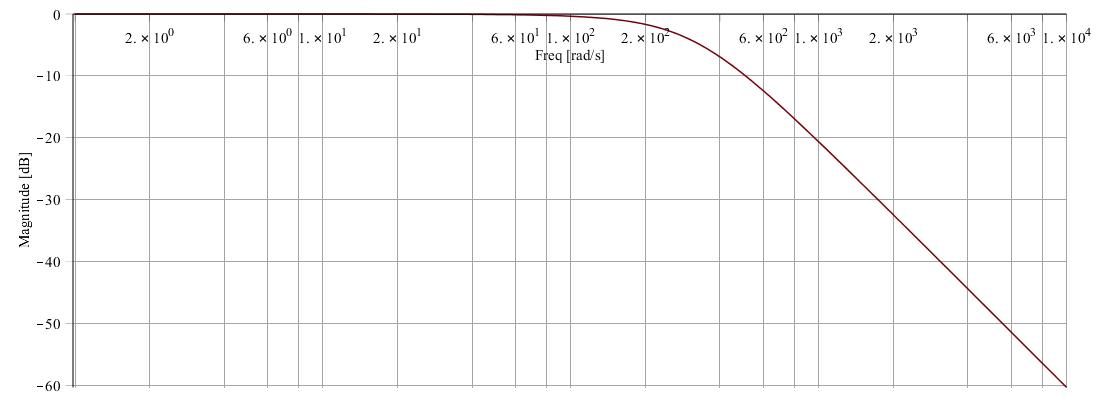
\includegraphics[scale=0.50]{bodeplot.PNG}
\caption{Bodeplot lavpasfilter}
\end{figure}

Bodeplottet bekræfter, at det er et lavpas filter. Der aflæses en knækfrekvens ved -3db til 269 rad/s $\approx$ 42,81Hz. Den beregnede knækfrekvens er blevet beregnet til 49,48 Hz. (Evt udregning i bilag)	
Dette er en relativ lille afvigelse. 

\subsubsection{Forstærker}

\section{Software}

\subsubsection{Trelagsmodellen}
Softwaren er opbygget af trelagsmodellen. 

